%
% teil2.tex -- Beispiel-File für teil2 
%
% (c) 2020 Prof Dr Andreas Müller, Hochschule Rapperswil
%
\section{Fraktale mit IFS 
\label{ifs:section:teil2}}
\rhead{Teil 2}
Wollen wir nun eine bestimmte Art anschauen, wie man Fraktale machen kann.
Zur Veranschaulichung dieser Methode nehmen wir das Sierpinski Dreieck.
\begin{figure}
	\centering
	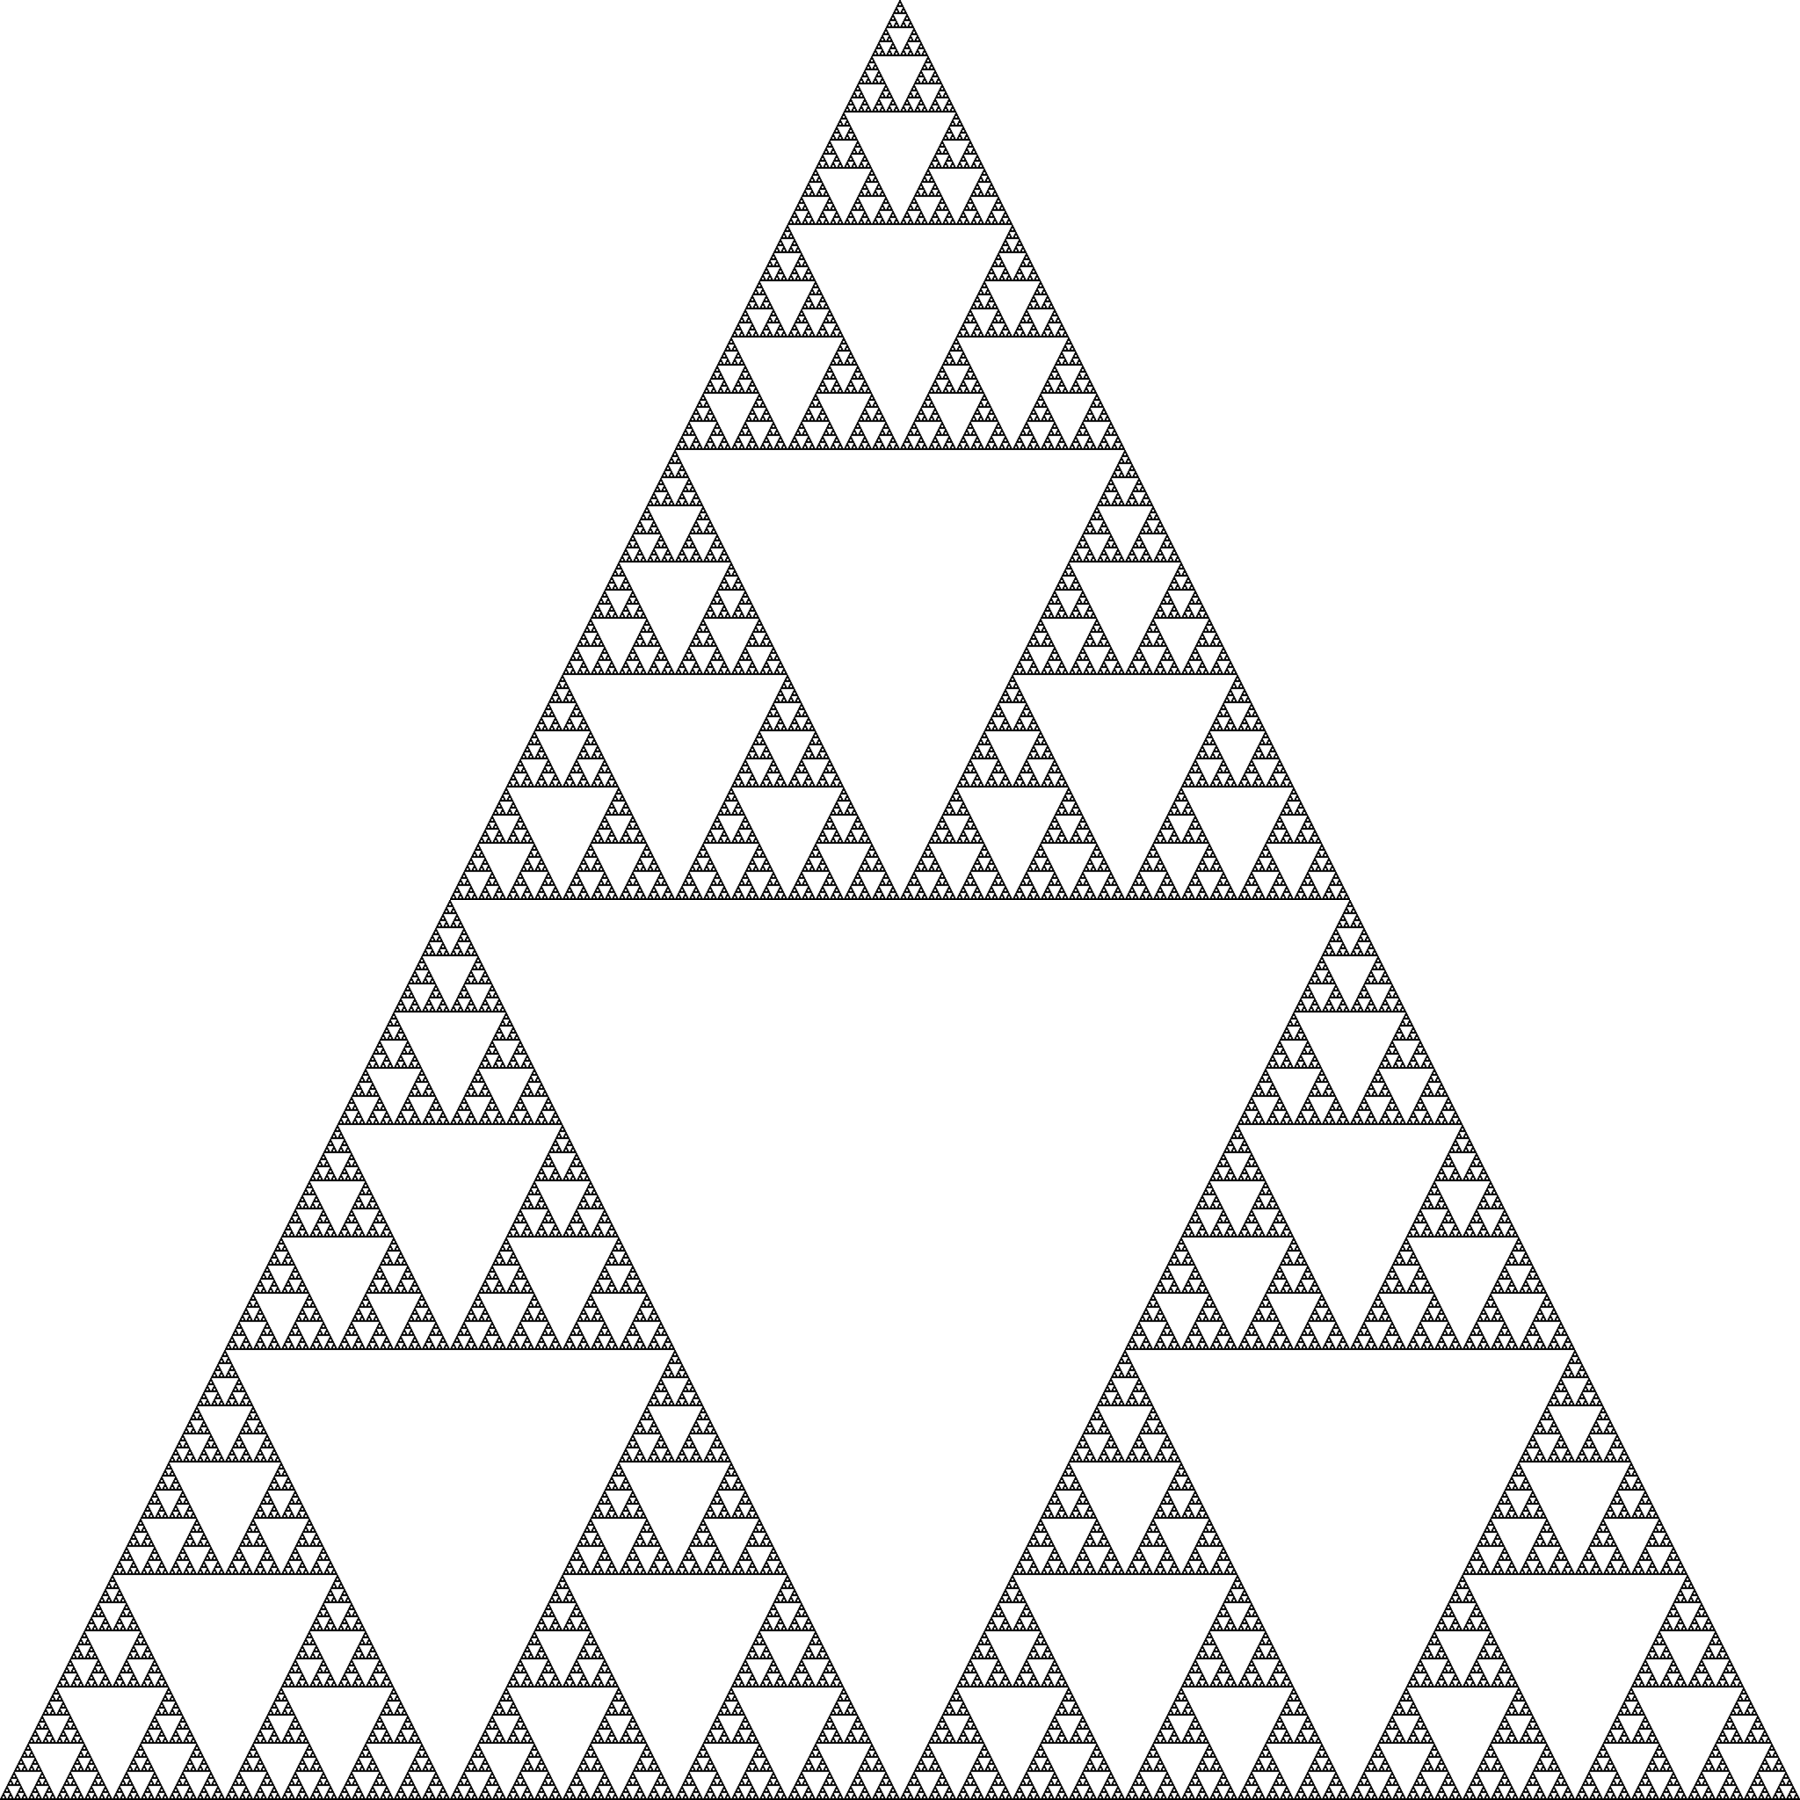
\includegraphics[width=0.5\textwidth]{papers/ifs/images/sierpinski}
	\caption{Sierpinski-Dreieck}
	\label{ifs:sierpinski10}
\end{figure}
Es besteht aus drei kleineren Kopien von sich selbst.
Es ist also ein Selbstähnliches Gebilde.
Diese Eigenschaft wollen wir uns zunutze machen.


Wir definieren das Dreieck mit Kantenlänge 1 als Menge $X$.
Ausserdem bestimmen wir drei Funktionen
\begin{align*}
	f_1(x,y)
	= 
	\begin{pmatrix}
		\frac{1}{2} & 0 \\
		0 & \frac{1}{2} \\
	\end{pmatrix}
	\begin{pmatrix}
		x\\
		y\\
	\end{pmatrix} 
	,\quad
	f_2(x,y)
	= 
	\begin{pmatrix}
		\frac{1}{2} & 0 \\
		0 & \frac{1}{2} \\
	\end{pmatrix}
	\begin{pmatrix}
		x\\
		y\\
	\end{pmatrix} 
	+
	\begin{pmatrix}
		\frac{1}{2} \\
		0
	\end{pmatrix}
	, \quad
	f_3(x,y)
	= 
	\begin{pmatrix}
		\frac{1}{2} & 0 \\
		0 & \frac{1}{2} \\
	\end{pmatrix}
	\begin{pmatrix}
		x\\
		y\\
	\end{pmatrix} 
	+
	\begin{pmatrix}
		\frac{1}{4} \\
		\frac{1}{2}
	\end{pmatrix},
\end{align*}
welche die gesamte Menge auf eine ihrer kleineren Kopien abbildet.
$f_1$ bildet das Dreieck auf das Teilstück unten links ab, $f_2$ auf das Teilstück unten rechts und $f_3$ auf das obere Teilstück.
Wendet man alle drei Funktionen auf das Sierpinski-Dreieck an
\begin{align*}
	X = \bigcup\limits_{i = 1}^{3} f_i(X),
\end{align*}
entsteht also wieder ein Sierpinski-Dreieck.
Man kann sogar noch einen Schritt weiter gehen, und sagen: Wenn wir die Funktionen auf eine beliebige Startmenge anwenden, konvergiert die Menge gegen das Sierpinski-Dreieck.
\begin{figure}	
	\centering
	\subfigure[]{
		\label{ifs:sierpconsta}
		
\includegraphics[width=0.25\textwidth]{papers/ifs/images/sierpinski1}}
	\subfigure[]{
		\label{ifs:sierpconstb}
		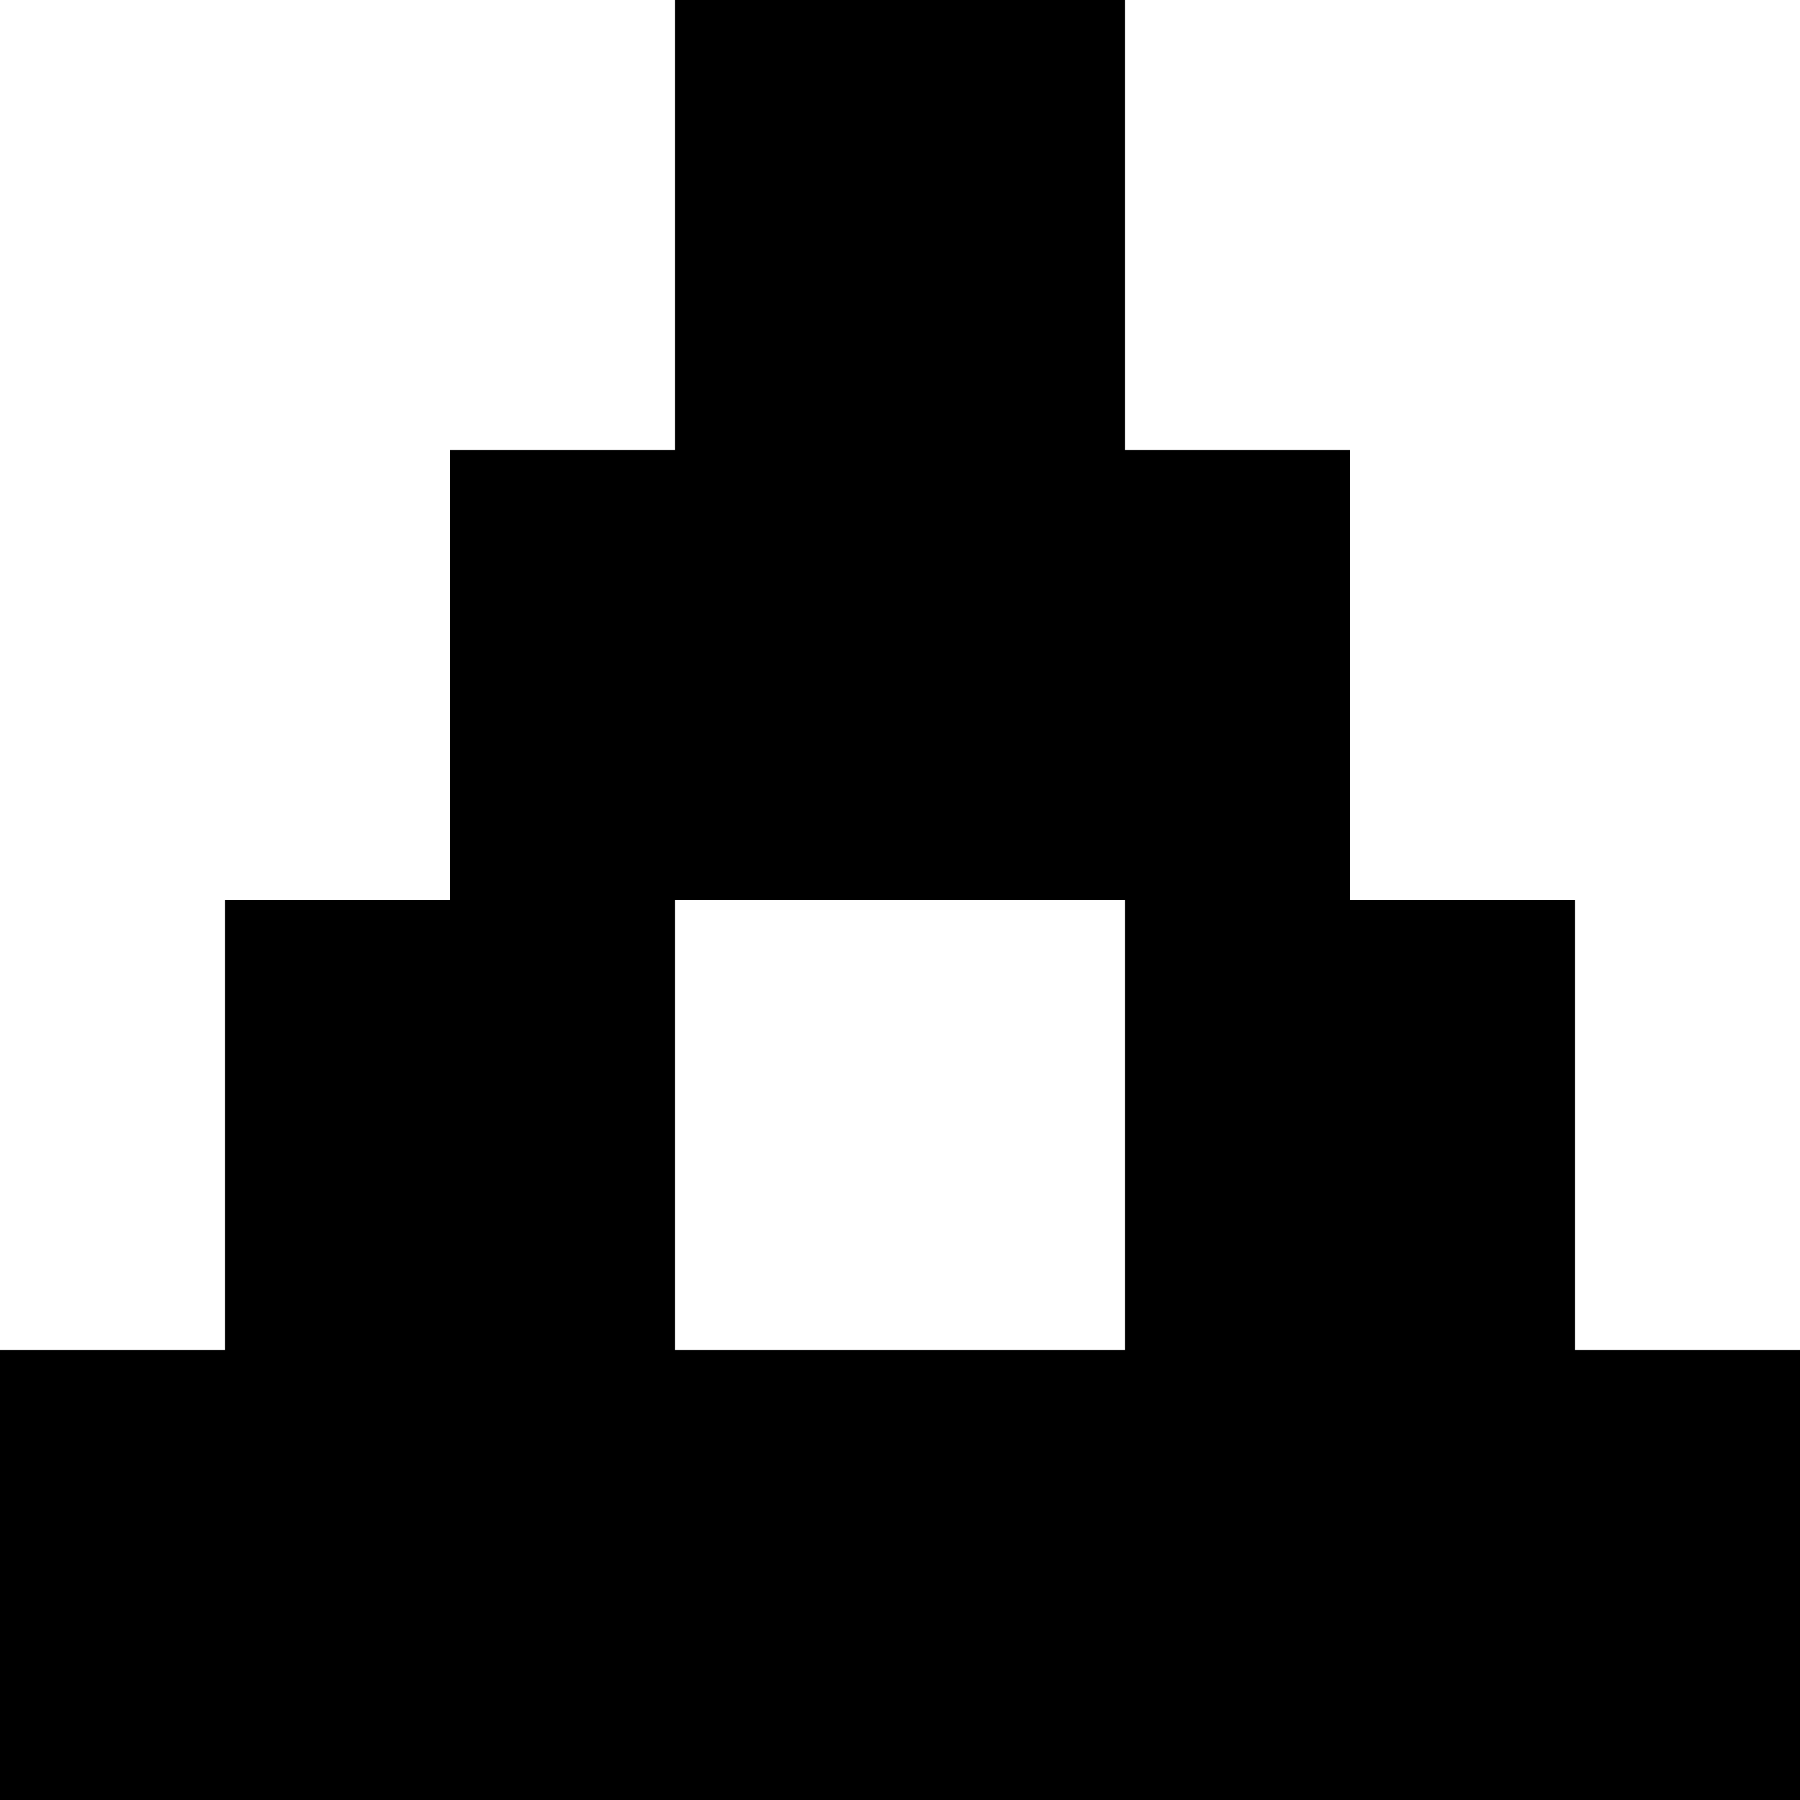
\includegraphics[width=0.25\textwidth]{papers/ifs/images/sierpinski2}} 
	\subfigure[]{
		\label{ifs:sierpconstc}
		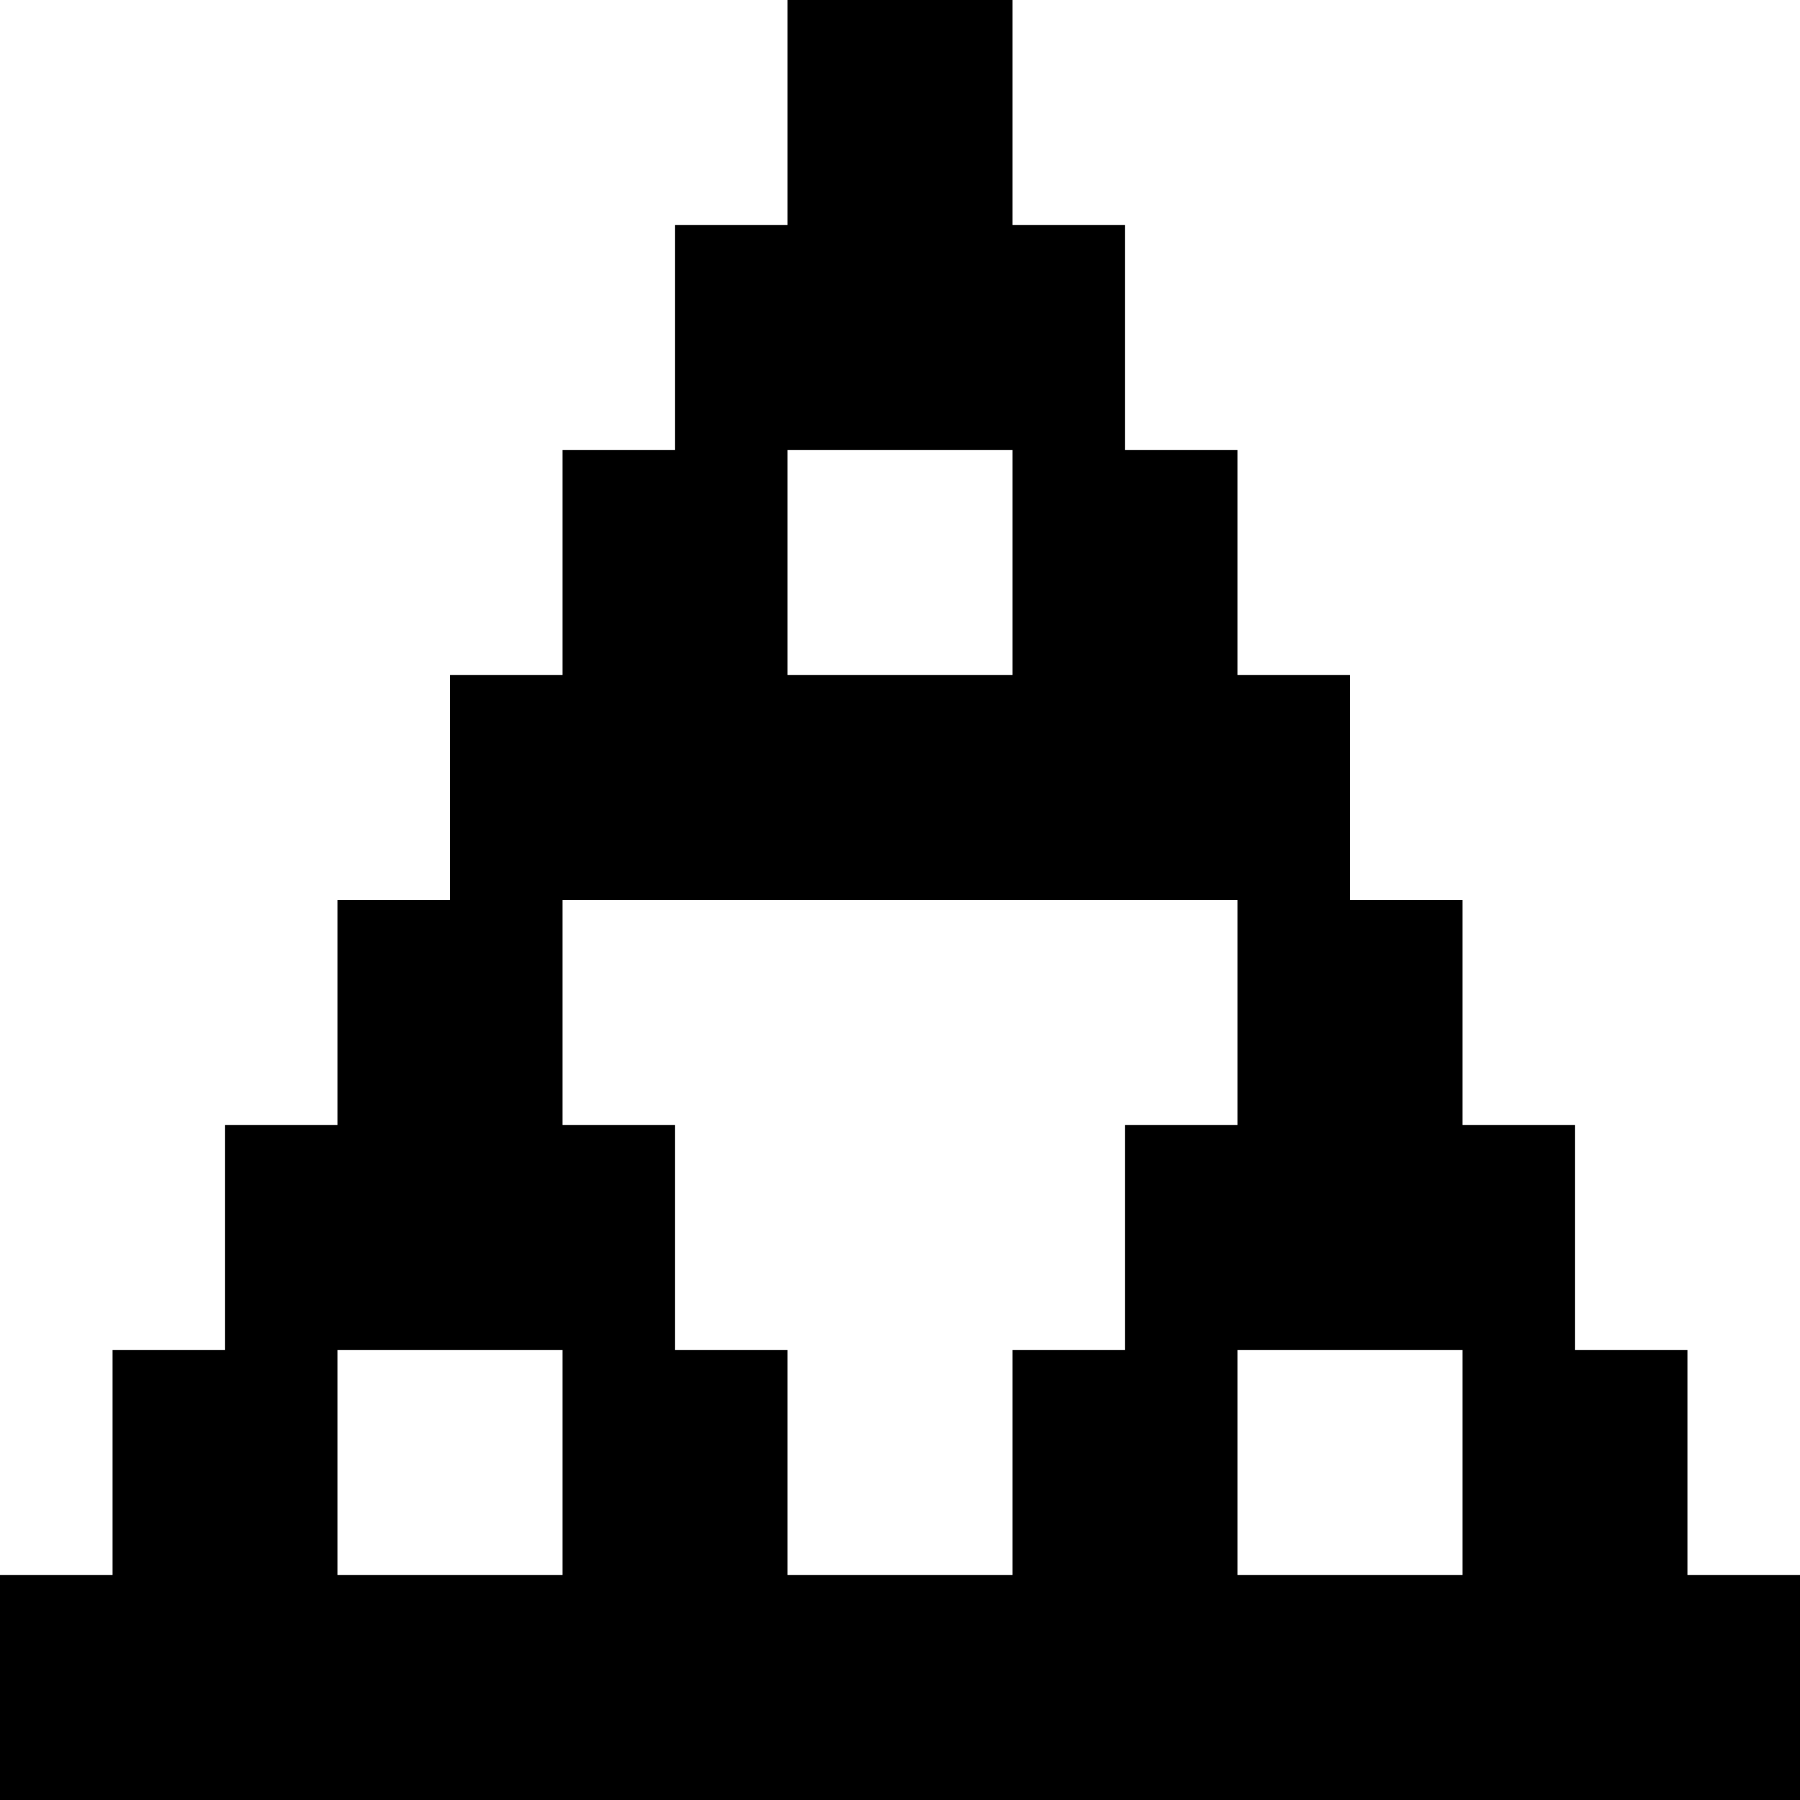
\includegraphics[width=0.25\textwidth]{papers/ifs/images/sierpinski3}}
	\subfigure[]{
		\label{ifs:sierpconstd}
		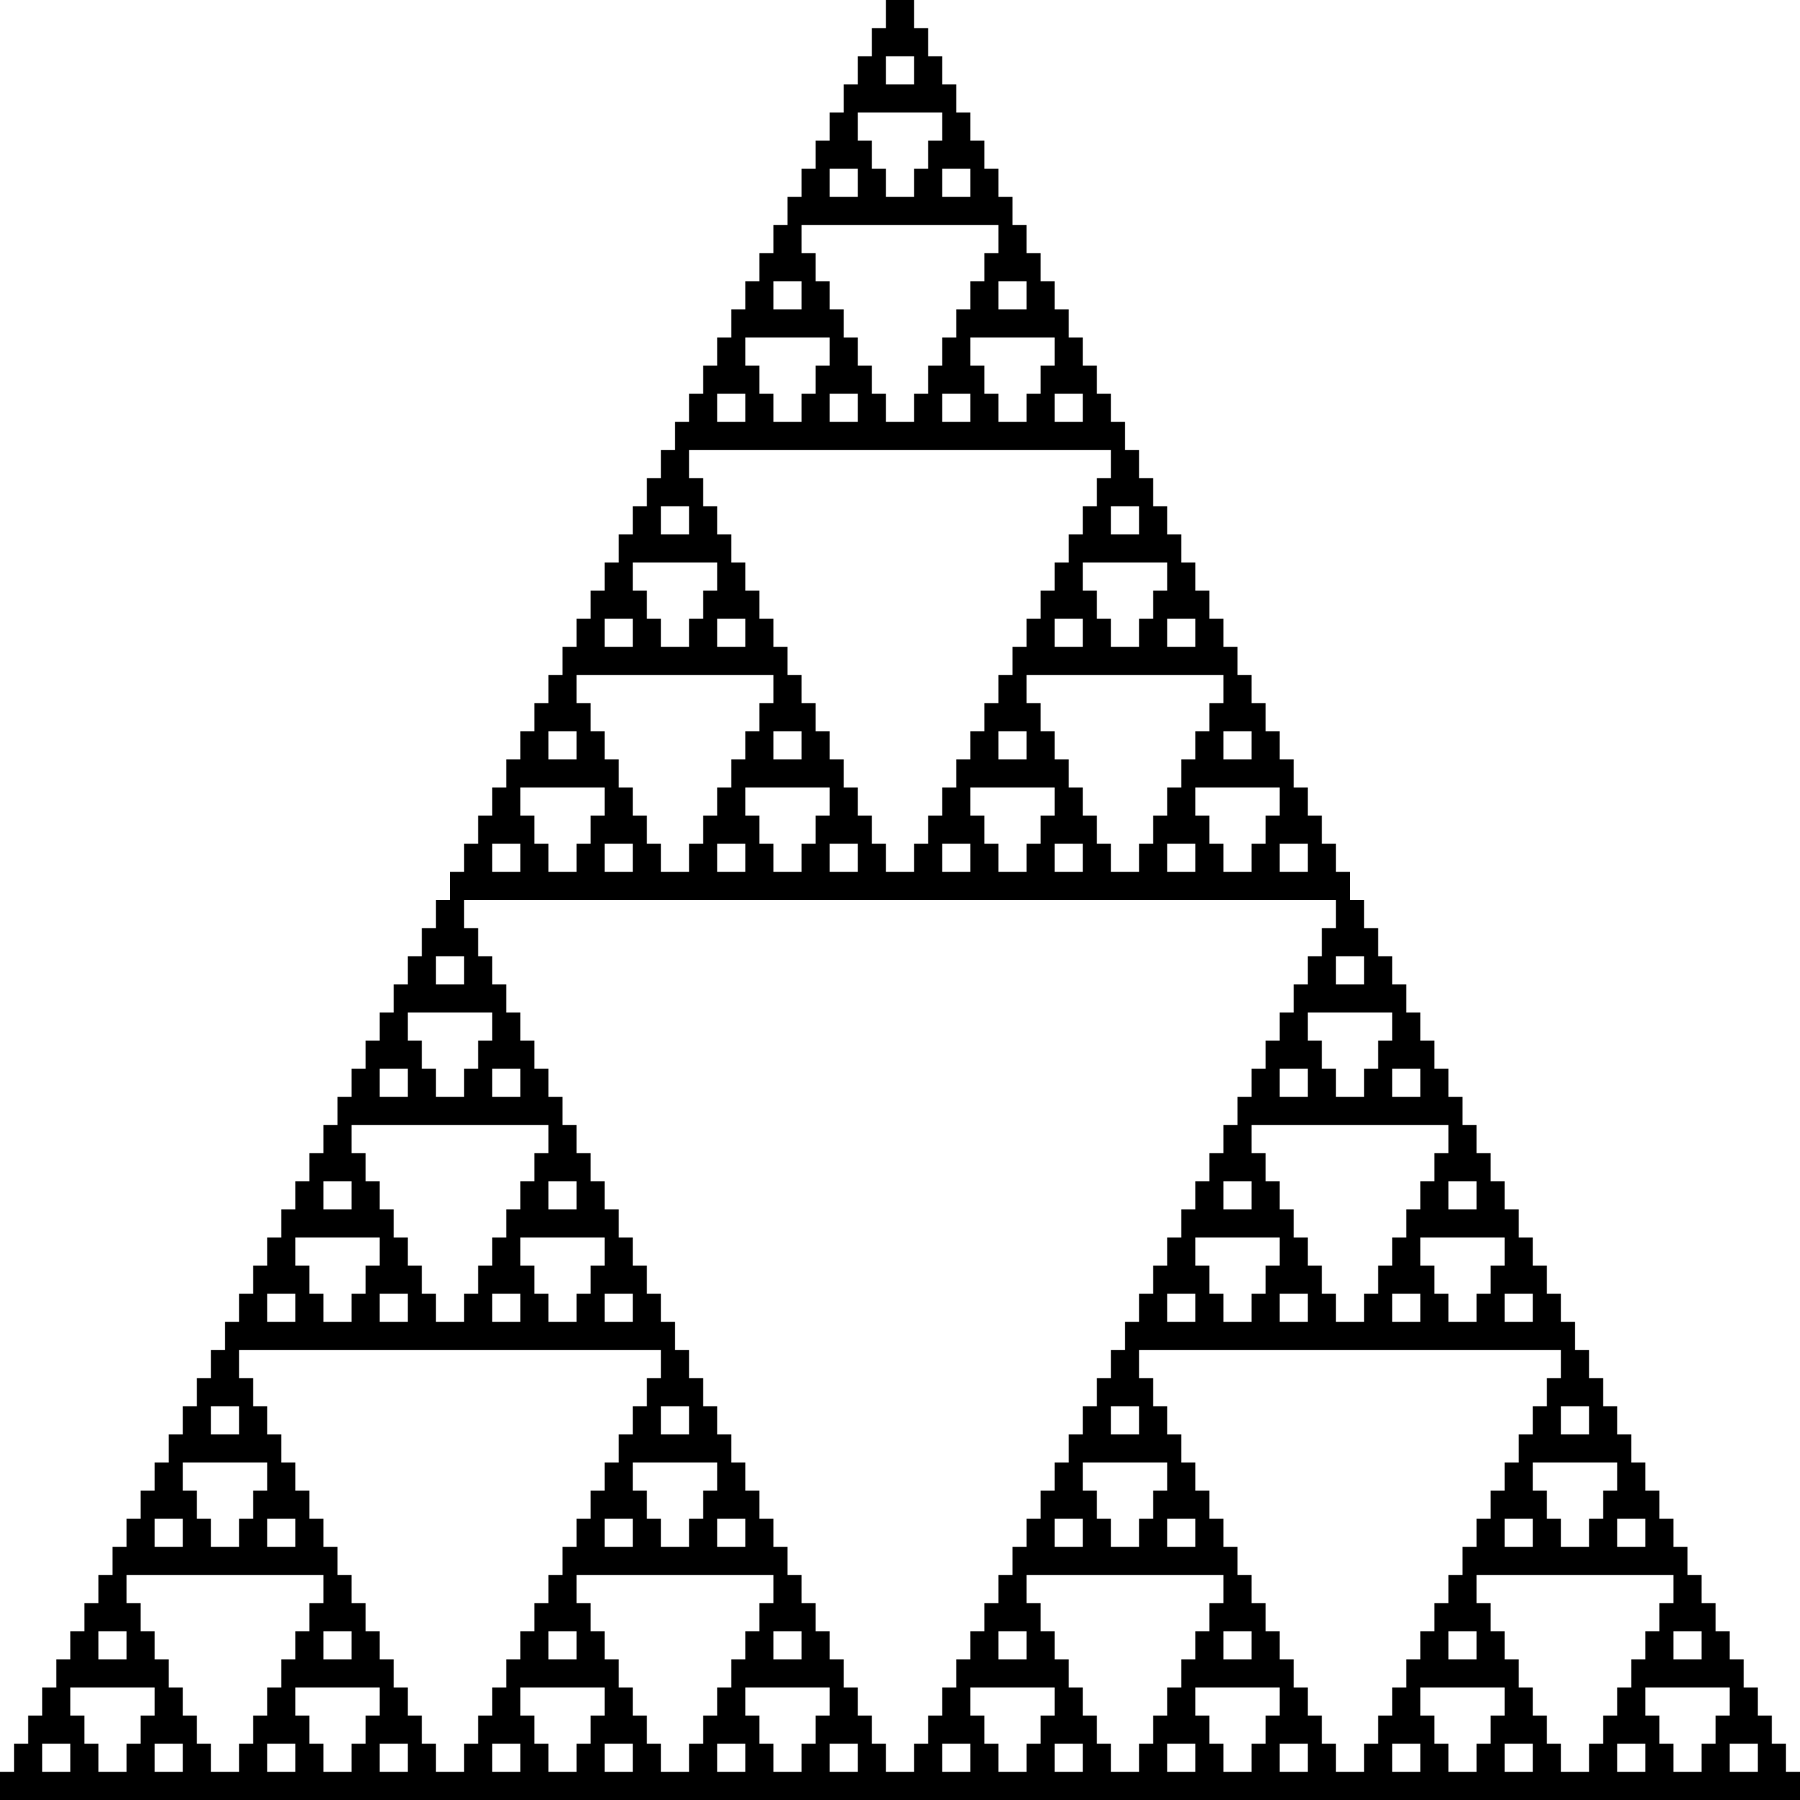
\includegraphics[width=0.25\textwidth]{papers/ifs/images/sierpinski6}}
	\caption{Konstruktion eines Sierpinski-Dreiecks mit einem Schwarzen Quadrat als Start\\
		(a) 1. Iteration (b) 2. Iteration (c) 3. Iteration (d) 5. Iteration}
	\label{ifs:sierpconst}
\end{figure}
Im Beispiel der Abbildung \ref{ifs:sierpconst} sehen wir, wie das Bild nach jeder Iteration dem Sierpinski-Dreieck ähnlicher wird.
Der Abstand zum Original wird immer kleiner, und konvergiert gegen null.

\subsection{Iterierte Funktionensysteme
\label{ifs:subsection:IteratedFunktionensysteme}}
In diesem Abschnitt wollen wir die Erkenntnis, wie wir aus einer beliebigen Menge ein Sierpinski-Dreieck generieren können, verallgemeinern.


$S_1,\dots,S_n$ sind Kontraktionen auf die Menge $D \subset \mathbb{R}^n$. Es gilt
\begin{align}
	|S_i(x) - S_i(y)| \leq c_i|x - y|
\end{align}
für jedes i mit einem $c_i < 1$.
Der Banachsche Fixpunktsatz besagt, dass für solche Kontraktionen ein Eindeutiges $A$ existiert, für das $S(A) = A$ gilt.
Den Beweis kann man in \cite{ifs:Rousseau2012} nachlesen.
Hat man nicht nur eine sondern mehrere Kontraktionen, dann existiert eine eindeutige kompakte Menge $F$ für die gilt
\begin{equation}
	F = \bigcup\limits_{i = 1}^{m} S_i(F).
\end{equation}
Weiter definieren wir die Transformation S auf kompakte Mengen $E$ ohne die leere Menge
\begin{equation}
	S(E) = \bigcup\limits_{i = 1}^m S_i(E).
	\label{ifs:transformation}
\end{equation}
Wird diese Transformation Iterativ ausgeführt, das heisst $S^0(E) = E, S^k(E) = S(S^{k-1}(E))$, gilt
\begin{equation}
	F = \bigcap\limits_{k = 1}^{\infty} S^k(E).
	\label{ifs:ifsForm}
\end{equation}
In Worte gefasst bedeutet das, dass jede Gruppe von Kontraktionen iterativ ausgeführt, gegen eine eindeutige Menge konvergiert.
Diese Menge ist auch als Attraktor eines IFS bekannt.
Der Beweis für die Existenz eines eindeutigen Attraktors ist in \cite{ifs:fractal-geometry} beschrieben. 

\subsection{Beispiel: Barnsley-Farn}
Der Barnsley-Farn, Abbildung \ref{ifs:farn}, ist ein Beispiel eines Fraktal, welches mit einem IFS generiert werden kann.
Wie man schnell erkennen kann, besteht der Farn aus Blättern, welche eine grosse Ähnlichkeit zum ganzen Farn haben.
Die vier affinen Transformationen
\begin{align}
	& {S_1(x,y)}
	= 
	\begin{pmatrix}
		0 & 0 \\
		0 & 0.16 \\
	\end{pmatrix}
	\begin{pmatrix}
		x\\
		y\\
	\end{pmatrix}, \quad &
	{S_2(x,y)}
	&= 
	\begin{pmatrix}
		0.85 & 0.04 \\
		-0.04 & 0.85 \\
	\end{pmatrix}
	\begin{pmatrix}
		x\\
		y\\
	\end{pmatrix} 
	+
	\begin{pmatrix}
		0 \\
		1.6
	\end{pmatrix}\\
	& {S_3(x,y)}
	= 
	\begin{pmatrix}
		0.2 & -0.26 \\
		0.23 & 0.22 \\
	\end{pmatrix}
	\begin{pmatrix}
		x\\
		y\\
	\end{pmatrix} 
	+
	\begin{pmatrix}
		0 \\
		1.6
	\end{pmatrix}, \quad &
	{S_4(x,y)}
	&= 
	\begin{pmatrix}
		-0.15 & 0.28 \\
		0.26 & 0.24 \\
	\end{pmatrix}
	\begin{pmatrix}
		x\\
		y\\
	\end{pmatrix} 
	+
	\begin{pmatrix}
		0 \\
		0.44
	\end{pmatrix}\\
	\label{ifs:farnFormel}
\end{align}
, welche für die konstruktion des Farns benötigt werden sind in der Abbildung \ref{ifs:farncolor} farblich dargestellt.
Das gesamte Farnblatt ist in der schwarzen Box.
Auf diese werden die Transformationen angewendet
$S_1$ erstellt den Stiel des Farnblattes (rot).
Die Transformation bildet das Gesamte Blatt auf die Y-Achse ab.
$S_2$ (grün) erstellt den Hauptteil des Farnes. 
Sie verkleinert und dreht das gesamte Bild und stellt es auf das Ende des Stiels aus $S_1$.
$S_3$ bildet das gesamte Blatt auf das blaue Teilblatt unten Links ab.
$S_4$ spiegelt das Blatt und bildet es auf das magentafarbene Teilblatt ab.  
\subsection{Erzeugung eines Bildes zu einem IFS}
Es gibt zwei verschiedene Methoden um das Bild zu einem IFS zu erzeugen.
Die erste Methode ist wahrscheinlich die intuitivste. 
Wir beginnen mit einm Startbild, zum Beispiel ein Schwarzes Quadrat, und bilden dieses mit den affinen Transformationen des IFS ab.
Das neue Bild, dass entsteht, ist die nächste Iterierte.
Dieses wird wieder mit den Transformationen abgebildet.
Wir wiederholen den letzten schritt, bis wir zufrieden mit der neusten Iterierten sind.

Diesen Vorgang haben wir beim Sierpinski-Dreieck in Abbildung \ref{ifs:sierpconst} gebraucht.
In Abbildung \ref{ifs:sierpinski10} ist die zehnte Iterierte zu sehen.
Weitere Iterationen hätten in dieser Darstellungsgrösse kaum mehr einen Unterschied gemacht.


Die zweite Methode ist das Chaosspiel \cite{ifs:chaos}. 
Bis jetzt wurde immer davon gesprochen, die Transformationen auf die gesamte Menge anzuwenden.
Bei komplizierteren IFS welche viele Iterationen brauchen, bis man den Attraktor erkennen kann, ist die erste Methode ziemlich rechenintensiv.
Beim Chaosspiel werden die Transformationen nicht auf die Menge angewendet, sondern nur auf einen einzelnen Punkt.
Der Startpunkt kann dabei ein beliebiger Punkt in $E$ sein.
Es wird bei jedem Iterationsschritt nur eine Transformation, welche zufällig gewählt wurde, angewendet.
Da, wie wir beim Barnsley-Farn gut sehen, nicht jede Transformation gleich viel des Bildes ausmacht, werden diese beim Chaosspiel gewichtet.
Je mehr eine Transformation kontrahiert, desto weniger Punkte braucht es um die resultierende Teilabbildung darzustellen.
Im Fall des Barnsley-Fern wird $S_1$ in $1\%$, $S_2$ in $85\%$ und $S_3 \& S_4$ in $7\%$ der Iterationen ausgeführt.
Wir sehen auch in Abbildung \ref{ifs:farncolor} gut, dass der rote Stiel, $S_1$, einiges weniger Punkte braucht als der grüne Hauptteil des Blattes, $S_2$.

In Abbildung \ref{ifs:farnNoWeight} wurden die vier gleich stark gewichtet.
Man sieht, dass trotzt gleich vieler Iterationen wie in Abbildung \ref{ifs:farn}, der Farn nicht so gut abgebildet wird.

Am besten sieht man den Effekt einer schlechten Gewichtung in Abbildung \ref{ifs:farnrightWeight}.
Hier wurde $S_4$, welches für das rechte untere Teilblatt zuständig ist, mit nur $1\%$ statt $7\%$ gewichtet.
Man sieht, wie sich der Mangel an Punkten auf die anderen Abbildungen das Farnblattes auswirkt.
In jeder Kopie des ganzen Farns fehlen die Punkte für dieses rechte untere Teilblatt.



\begin{figure}	
	\centering
	\makebox[\textwidth][c]{
		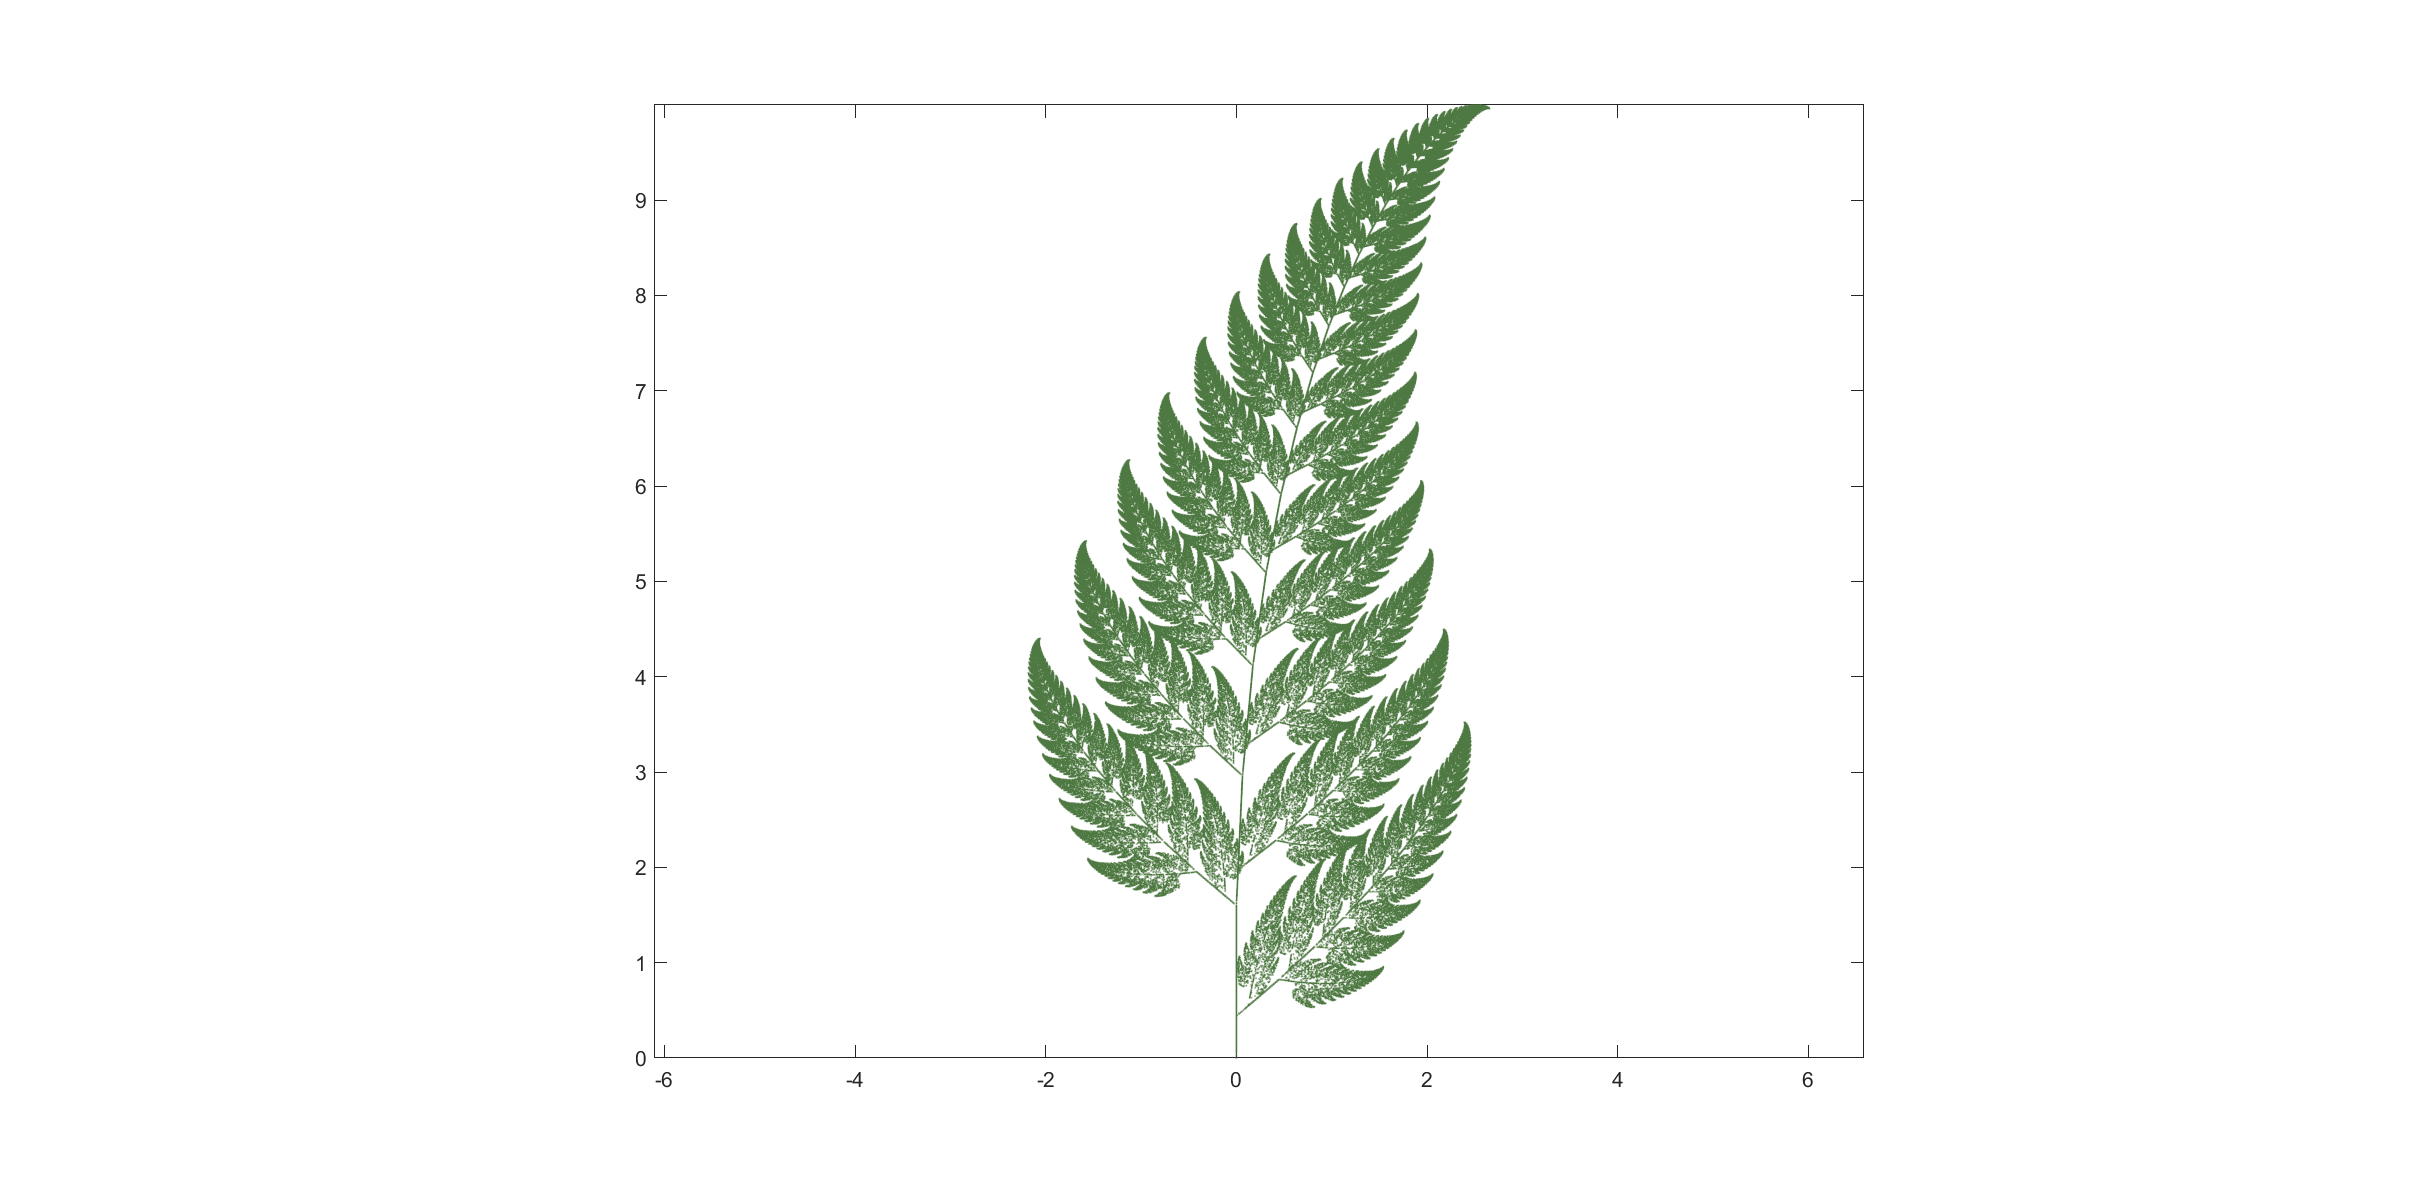
\includegraphics[width=1.4\textwidth]{papers/ifs/images/farn}}
	\caption{Barnsley-Farn}
	\label{ifs:farn}
\end{figure}
\begin{figure}
	\centering
	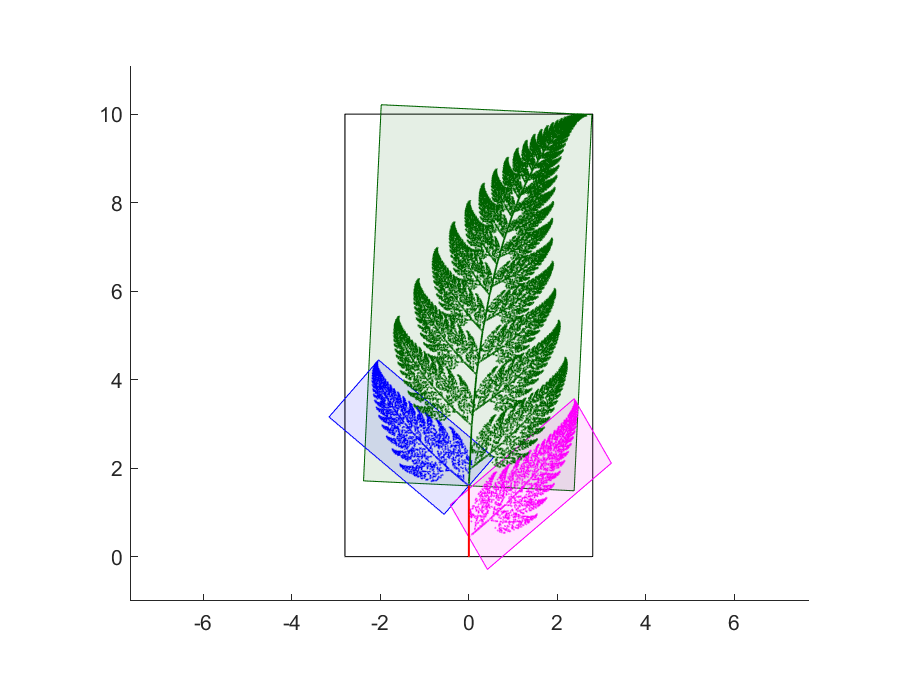
\includegraphics[width=\textwidth]{papers/ifs/images/farncolor2}
	\caption{Vier Transformationen des Barnsley-Farn in unterschiedlichen Farben}
	\label{ifs:farncolor}
\end{figure}

\begin{figure}	
	\centering
	\subfigure[]{
		\label{ifs:farnNoWeight}
		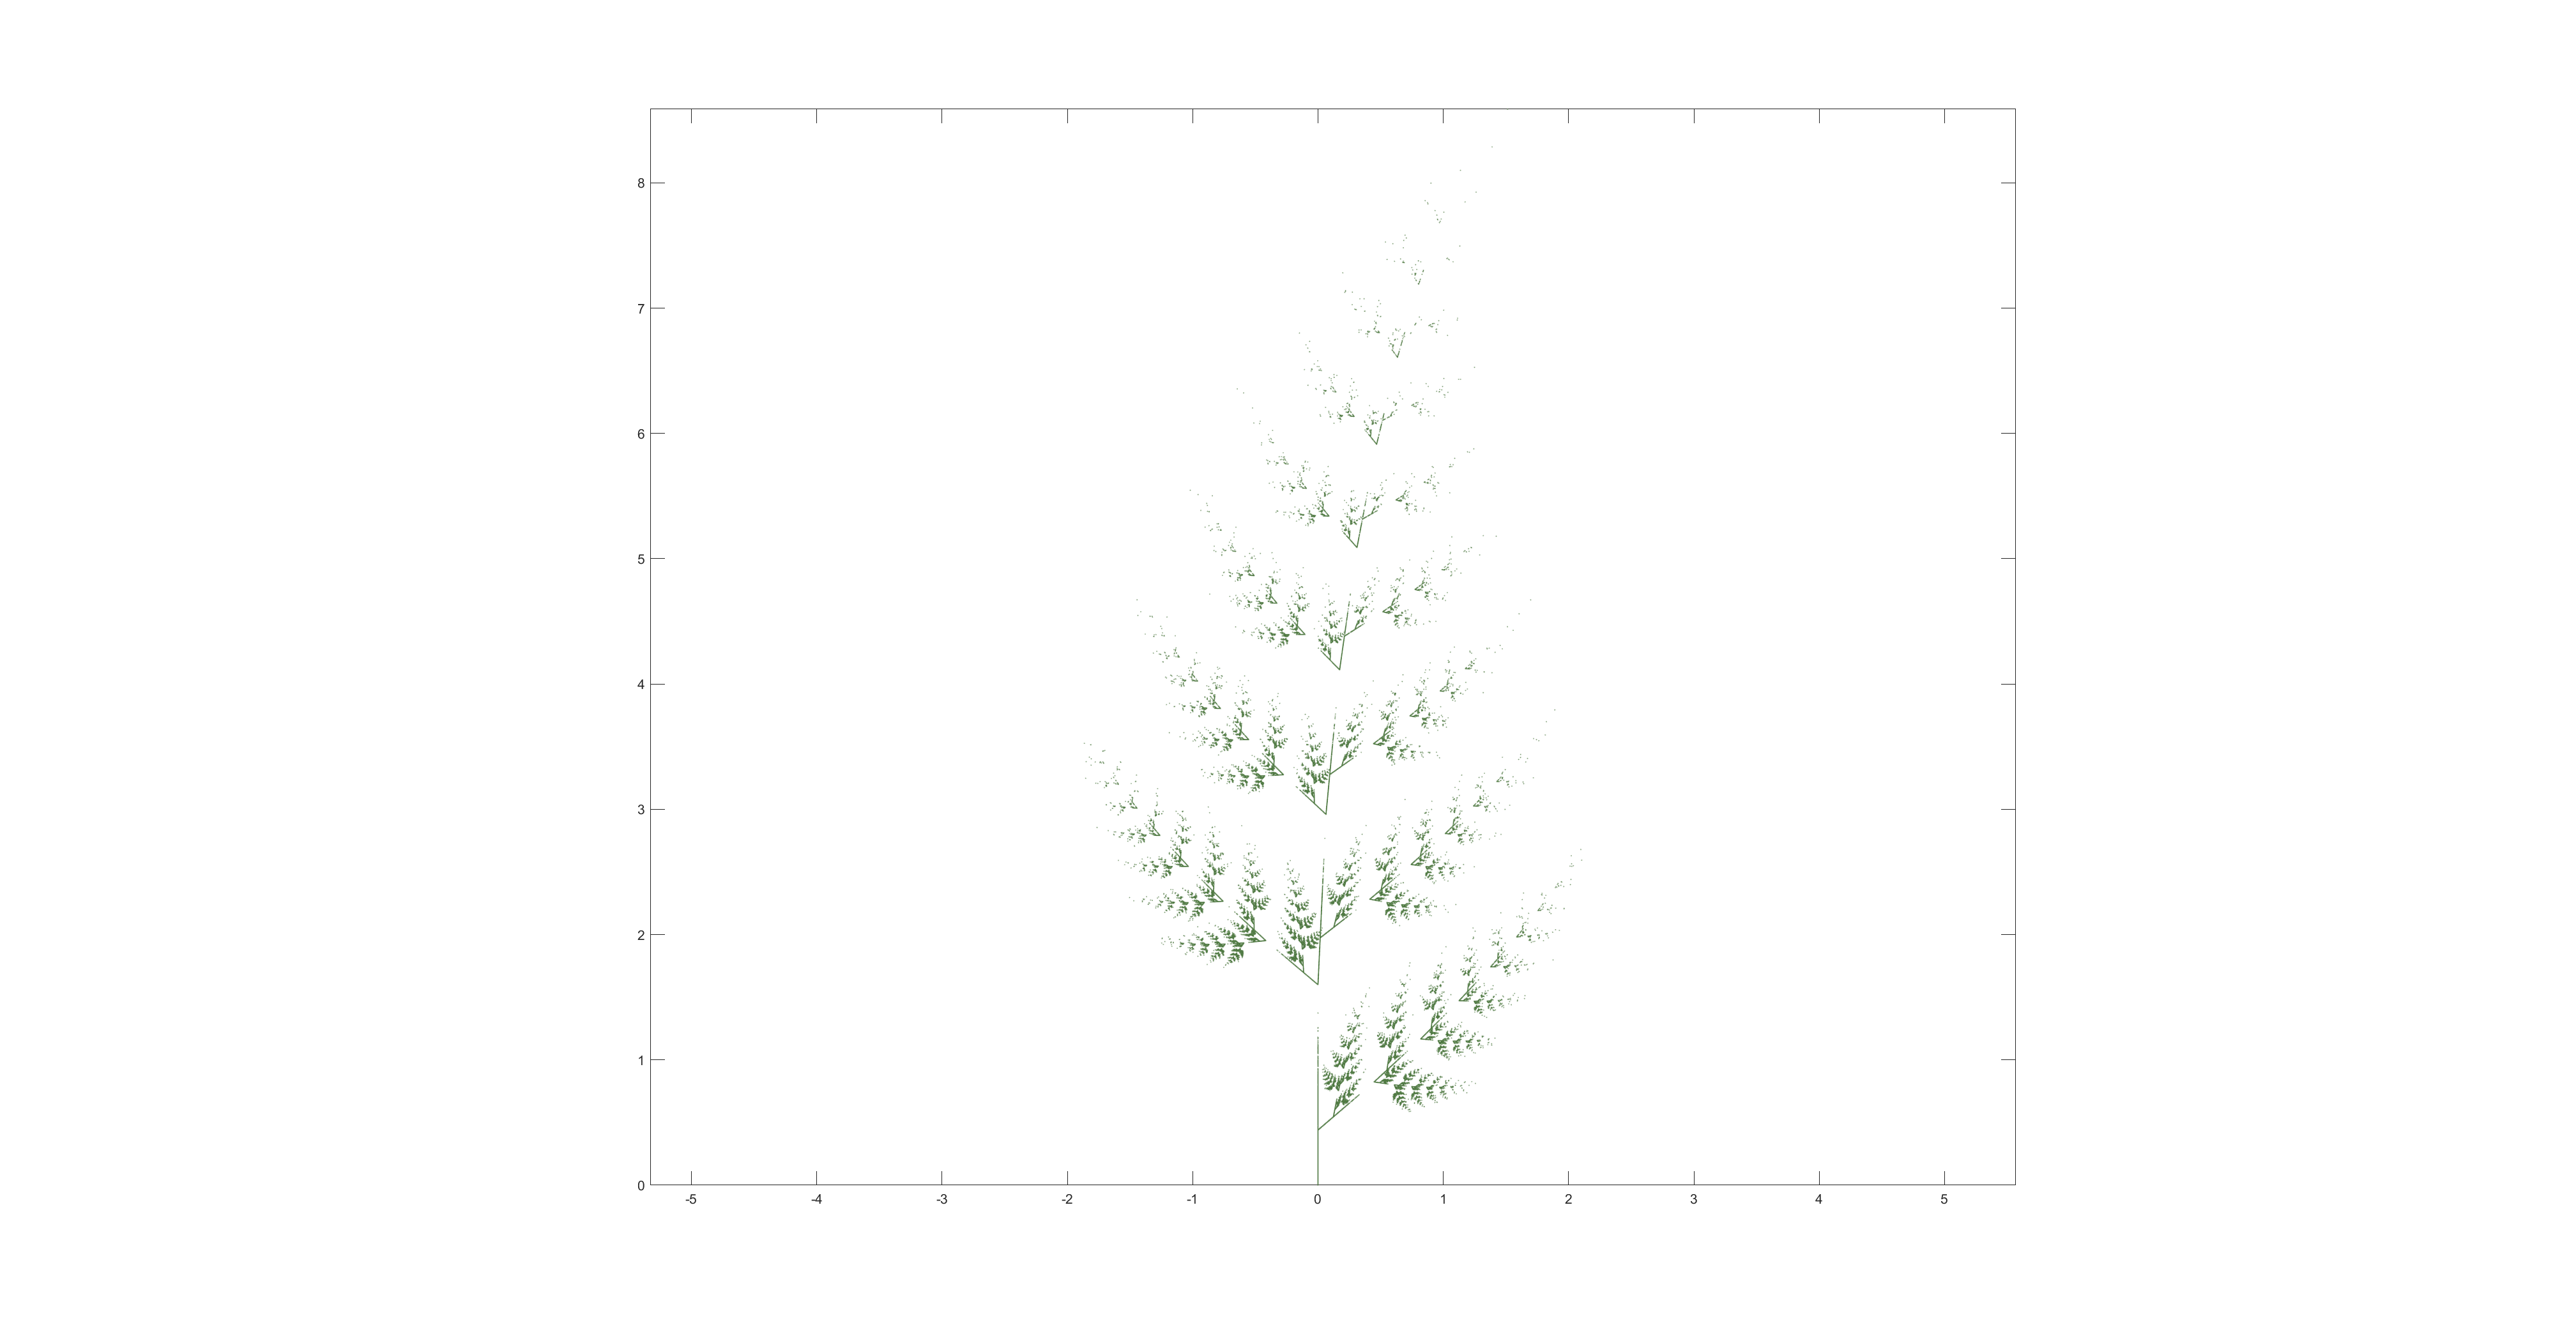
\includegraphics[width=0.45\textwidth]{papers/ifs/images/farnnotweight}}
	\subfigure[]{
		\label{ifs:farnrightWeight}
		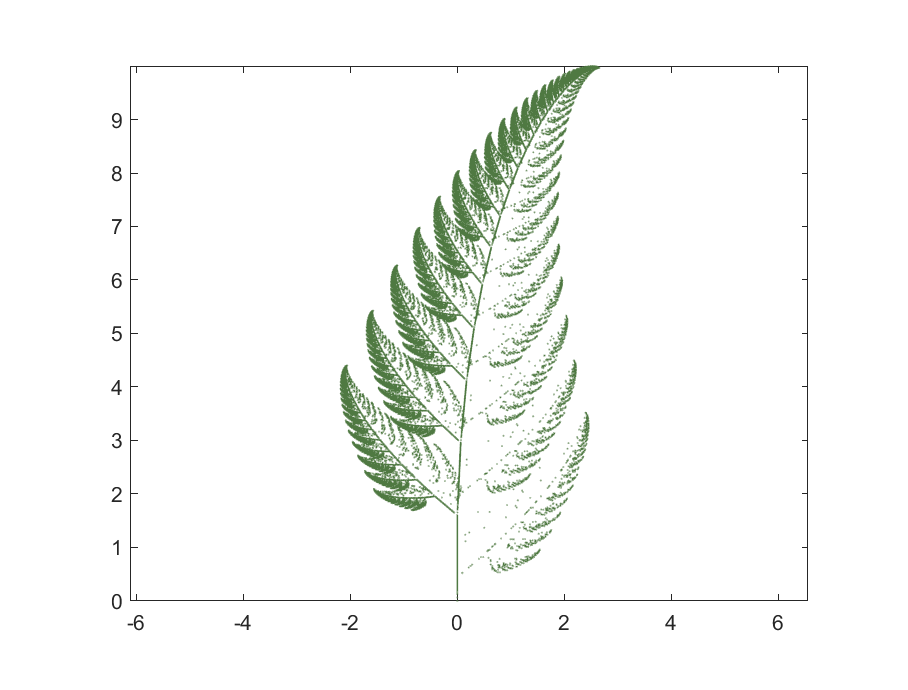
\includegraphics[width=0.45\textwidth]{papers/ifs/images/farnrightwight}}
	\caption{(a) Chaosspiel ohne Gewichtung (b) $S_4$ zu wenig gewichtet}
	\label{ifs:farnweight}
\end{figure}
